\documentclass[10pt]{article}
\usepackage{graphicx}
\graphicspath{ {./images/} }
\usepackage{titlesec}
\usepackage{amssymb,amsthm,amsmath,commath}
%\pagestyle{empty}
\textwidth = 7 in\textheight = 9.5 in\oddsidemargin = -.25 in\evensidemargin = -.25 in\topmargin = -.25 in\headheight = 0.0 in\headsep = 0.0 in\parskip = 0.2in\parindent = 0.0in
\newcommand{\ds}{\displaystyle}
\newenvironment{rcases}
  {\left.\begin{aligned}}
  {\end{aligned}\right\rbrace}

\title{Independent Study in Differential Equations}
\date{2018\\Fall Semester}
\author{Melissa Wallace\\Math Department, Winthrop University\\Dr. Trent Kull}

\begin{document}
\maketitle
%\renewcommand{\arraystretch}{1.2}

\section{Introduction to Material}
    ``A differential equation is an equation that contains one or more derivatives of an unknown function." - W. Trench. %make sure to actually site this later.
    The purpose of this course is to provide background before entering into the the profession of teaching. By not having taken a differential equations course at Winthrop University and needing 2 credit hours, the purpose is to obtain more knowledge and preparations in order to teach Calculus one day. %will probably add to this later once things get rolling
    It has begun as a crash course version of the standard course at Winthrop and will shift into applying Linear Algebra to the course material as well.
    
    \subsection{Basic Content Introduction}
        
    
\section{First Order Equations}
    Many differential equations derived from real world situations cannot be solved, but we will approach the ones that can be solved in this course, and the ways to solve those.\\
    
    Linear equations are the simplest form of first order equations as they can be solved using variation of parameters. A first order equation is called linear if it takes on the form $$y'=p(x)y=f(x).$$ The equation is otherwise counted as non-linear. 
    
    Begin by considering equations that can solve the following problem where a function is equal to its first derivative: $$f(x)=f'(x).$$
    The solutions will take on the form: $0, e^x, 2e^x, 3e^x, \pi e^x$. Thus we arrive at a general solution to these equations being: $$f(x)=ce^x \text{ where } c\in\mathbb{R}.$$
    
    Similarly, consider the solution to an equation where a function is equal to its second derivative: $$f(x)=f''(x).$$
    One solution to this problem looks as follows:
    \begin{eqnarray*}
        f_1(x)=\sin(x)\\
        f_1'(x)=\cos(x)\\
        f_1''(x)=\sin(x)
    \end{eqnarray*}
    It works similarly for $f(x)=\cos(x)$, or $f(x)=2\sin(x)$, $f(x)=-3\cos(x)$, or even $f(x)=2\sin(x)-3\cos(x)$. Therefore, we arrive at a general solution to these equations being: $$f(x)=c_1\sin(x)+c_2\cos(x) \text{ where } c_1,c_2\in\mathbb{R}.$$
    \\
    
%is the following actually a practice problem??? check this.
    Practice: let $x'(t)=2e^{2t}-2e^{-2t}$ and $y'(t)=-10e^{-2t}+2e^{2t}$.
    
    \subsection{Separation of Variables}
        The first strategy for solving Linear First Order Equations that we will focus on is Separation of Variables. This process looks like: $$\frac{dy}{dt}=\frac{g(t)}{f(y)} \text{ with the resulting } \int{f(y)dy}=\int{g(t)dt}.$$
        Then $f(y)\frac{dy}{dt}=g(t)$ and we assume there exists an $F(y)$ such that $\frac{dF}{dy}=f(y)$.\\
        Then notice that:
        \begin{eqnarray*}
            g(t)        &=&\frac{dF}{dy}\frac{dy}{dt} \\
            \int{g(t)dt}&=&\int{\frac{dF}{dy}\frac{dy}{dt}dt}\\
            \int{g(t)dt}&=&\int{\frac{dF}{dt}dt}     \hspace{1cm}\text{by the Chain Rule.}\\
            \int{g(t)dt}&=&F[y(t)]\\
            \int{g(t)dt}&=&\int{f(y)dy}.
        \end{eqnarray*}
    
        Now for practice:
        \begin{enumerate}
            \item[1.] Solve $\frac{dy}{dx}=-\frac{x}{y}$ with the initial condition $y(1)=1$.\\
            Notice then that $g(x)=-x$ and $f(y)=y$.\\
            Then,
            \begin{eqnarray*}
                \int{ydy}&=&\int{-xdx}\\
                \frac{y^2}{2}&=&\int{-xdx}+c_1\\
                y^2&=&x^2+c_2\\
                y^2+x^2&=&c\\
                \text{Implementing the initial value:}\\
                y(1)^2+1^2&=&c\\
                1+1&=&c\\
                c&=&2\\
                \text{Thus:}\\
                x^2+y^2&=&2
            \end{eqnarray*}
    
            \item[2.] Solve $\frac{dy}{dx}=\frac{1}{(\frac{1}{y})}.$
            Notice that $g(x)=1$ and $f(y)=\frac{1}{y}$.\\
            \begin{eqnarray*}
                \int{\frac{1}{y}dy}&=&\int{1dx}\\
                e^{\ln{\mid{y}\mid}}&=&e^{x+c_1}\\
                \abs{y}&=&e^{x+c_1}\\
                \abs{y}&=&e^x e^{c_1}\\
                \abs{y}&=&e^x c_2\\
                y&=&e^x c\\
                y&=&ce^x
            \end{eqnarray*}
            
            \item[3.] Solve $\frac{dy}{dx}=2x$ with the initial condition $y(0)=4$ and the given $c=4$.\\
            \begin{eqnarray*}
                \int{\frac{dy}{dx}dx}&=&\int{2xdx}\\
                y(x)&=&x^2+c \hspace{1cm}\text{(general solution)}\\
                y(x)&=&x^2+4v\hspace{1cm}\text{(specific solution)}\\
            \end{eqnarray*}
        \end{enumerate}
    
    In general the solution for a First Order Differential Equation solved explicitly for $\frac{dy}{dx}$, $$\frac{dy}{dx}=f(y,t).$$
    
    \subsection{Applications - Cooling Problems????}
%introduce the subject here somewhere !!!
    
    $$T'(t)=-k[T(t)-R], k>0$$
    $$\text{initial conditions:  } k=1=R, T(0)=T_0$$

    \newpage
    
    \subsection{Direction Fields}
%include the handout before this in the binder.
    
    \begin{center}{\bf\large MATH 471\\Lab 1\\Direction Field Homework}\end{center}
        {\bf Problem 1} $y'=ty$
            \begin{center}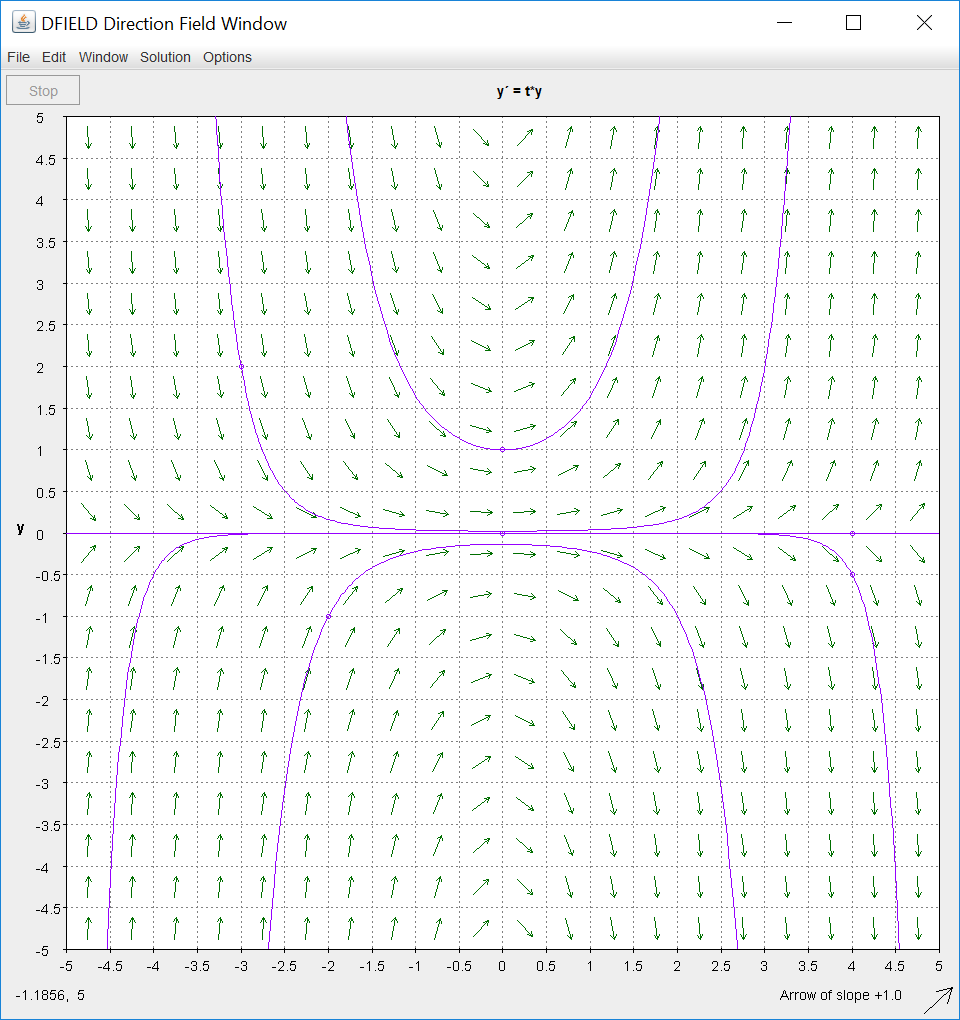
\includegraphics[scale=0.5]{lab1p3p1.PNG}\end{center}
        {\bf Problem 2} $y'=y^2-t^2$
            \begin{center}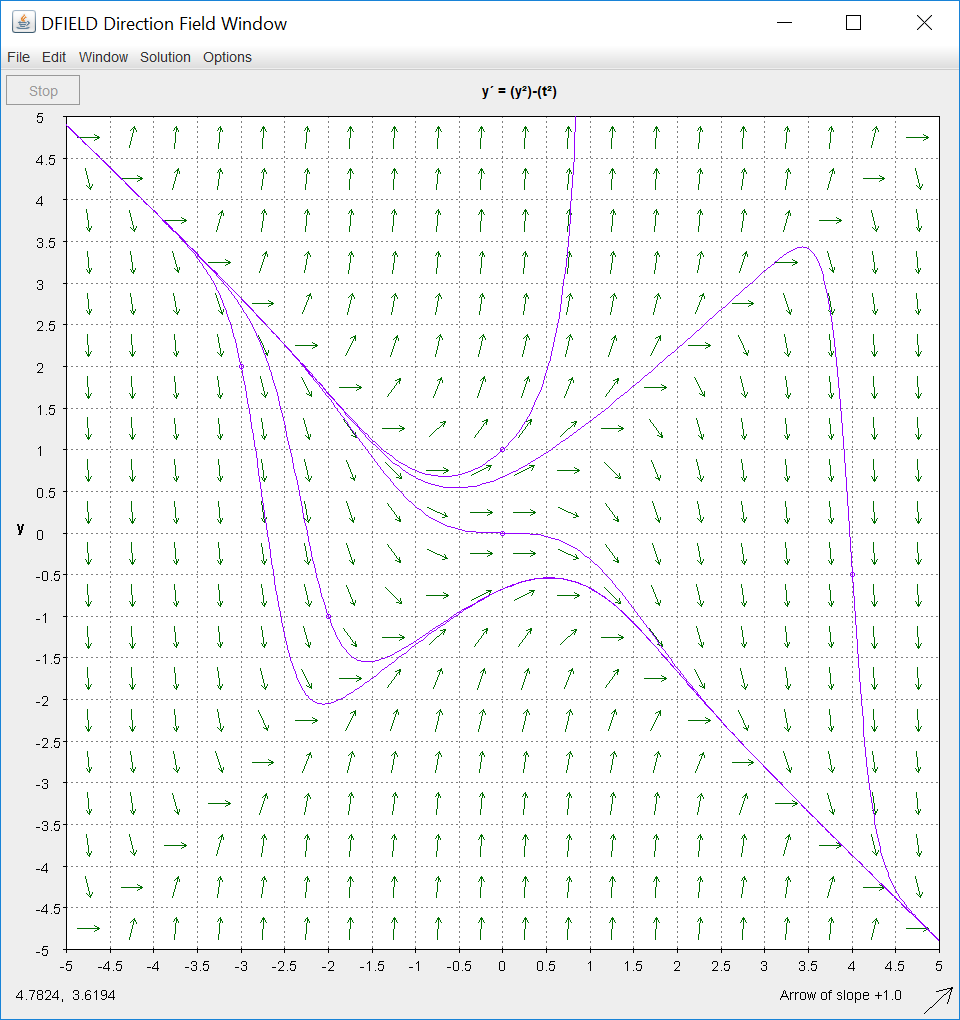
\includegraphics[scale=0.5]{lab1p3p2.PNG}\end{center}
        {\bf Problem 3} $y'=\frac{2ty}{1+y^2}$
            \begin{center}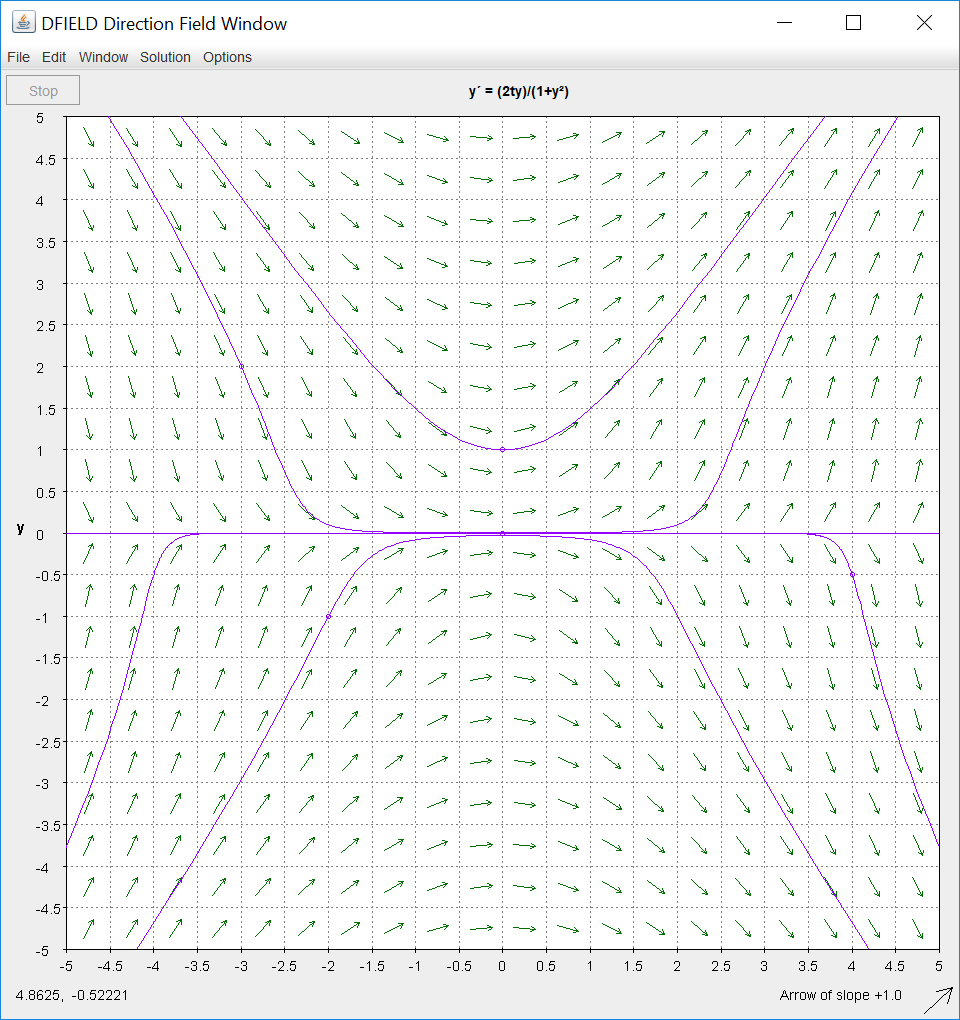
\includegraphics[scale=0.5]{lab1p3p3.PNG}\end{center}
        {\bf Problem 4} $y'=y(2+y)(2-y)$
            \begin{center}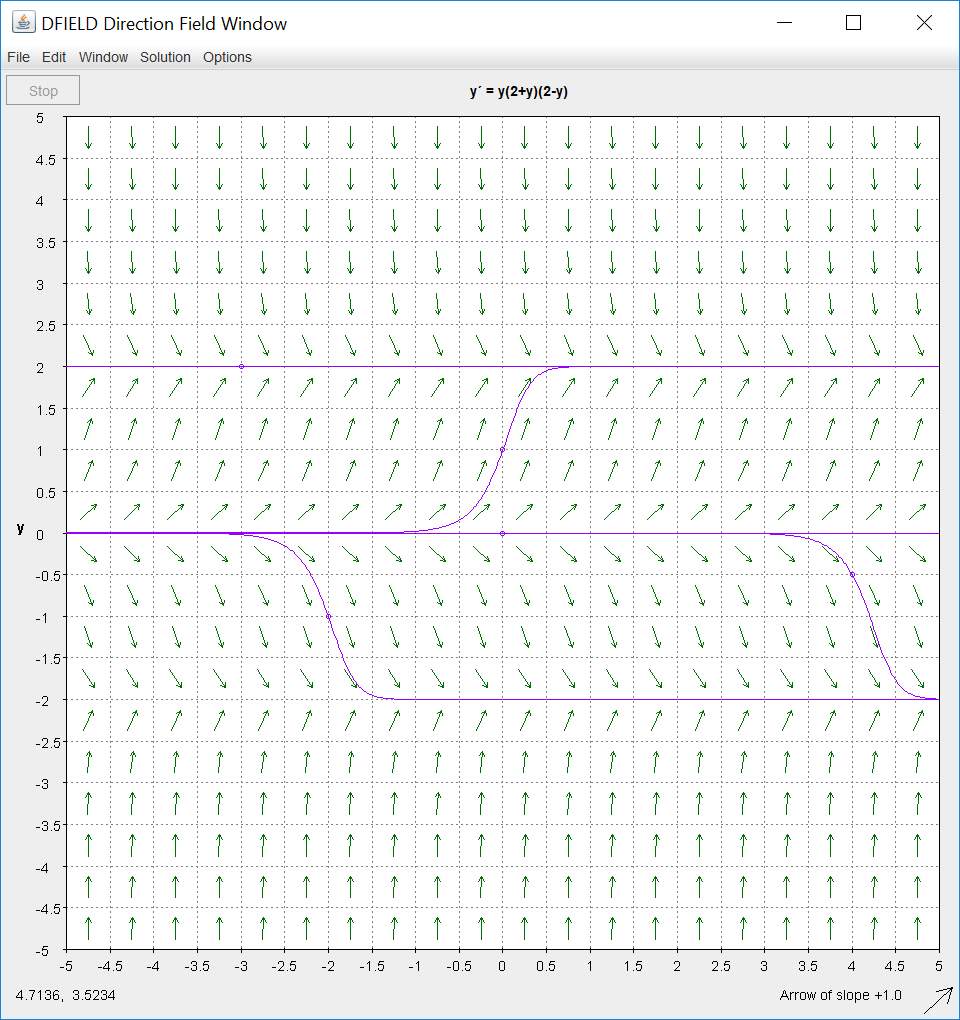
\includegraphics[scale=0.5]{lab1p3p4.PNG}\end{center}
        {\bf Problem 5} $y'+3y=8$
            \begin{enumerate}
                \item[a)] $y'=-3y+8$ \begin{center}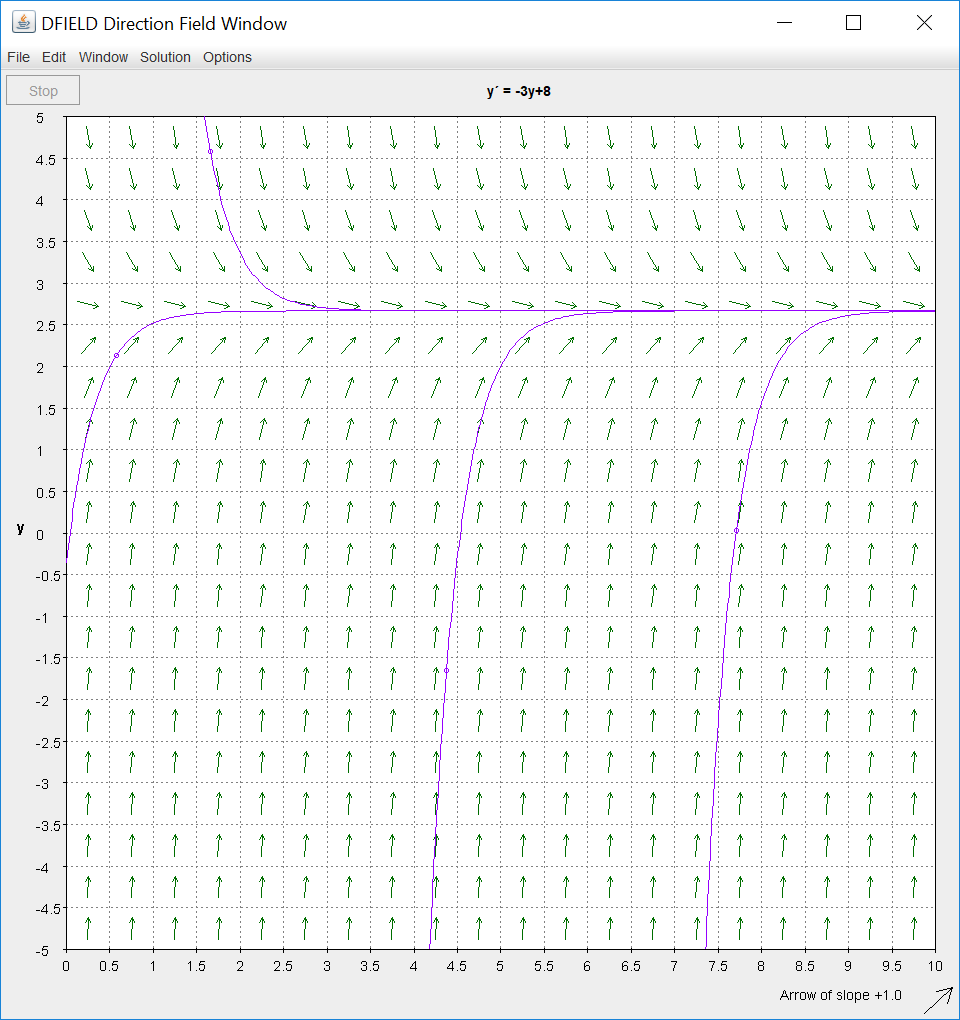
\includegraphics[scale=0.5]{lab1p3p5.PNG}\end{center}
                \item[b)] My conjecture for the limiting behavior as $t \rightarrow \infty$ is that $y$ will always follow the path to 2.55.
            \end{enumerate}
        {\bf Problem 6} $(1+t^2)y'+5ty=t$
            \begin{enumerate}
                \item[a)] $y'=\frac{t-5ty}{1+t^2}$ \begin{center}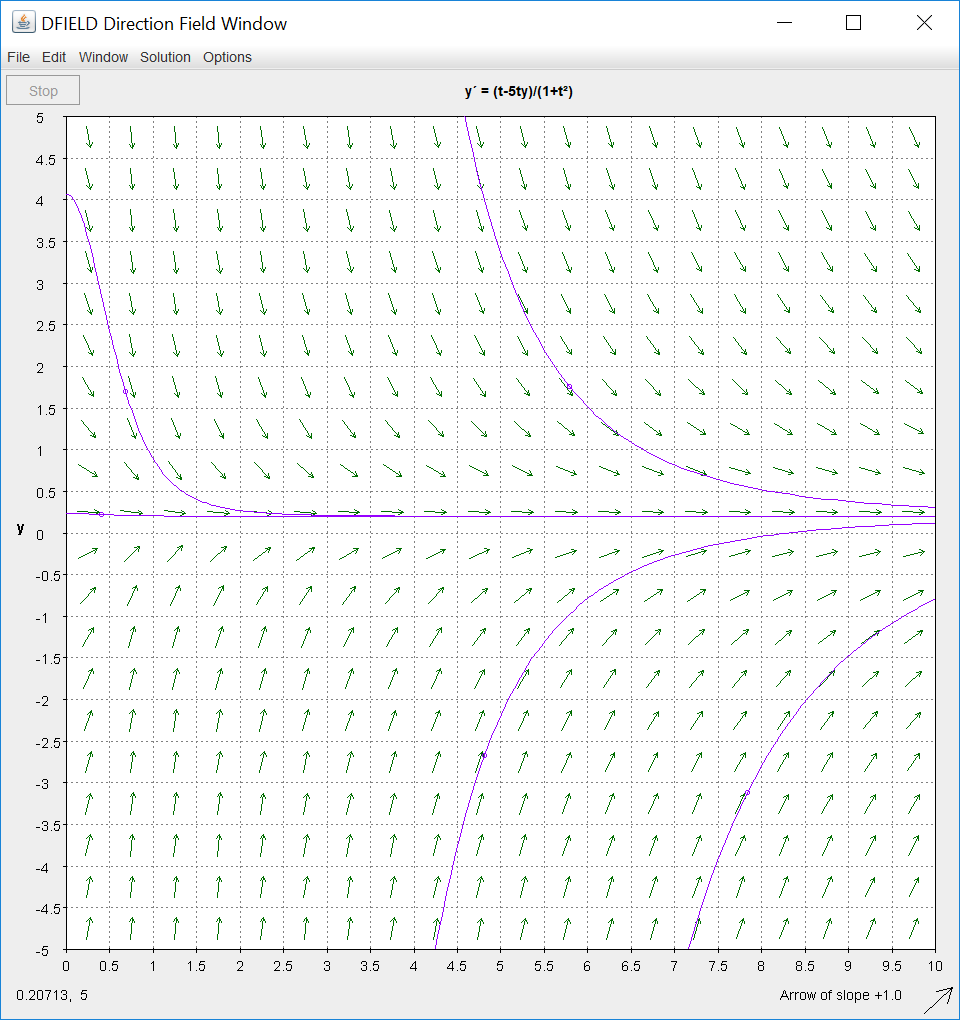
\includegraphics[scale=0.5]{lab1p3p6.PNG}\end{center}
                \item[b)] My conjecture for the limiting behavior as $t \rightarrow \infty$ is that $y=0.05$.
            \end{enumerate}
        {\bf Problem 7} $ty'+ty=15-y$
            \begin{enumerate}
                \item[a)] $y'=\frac{15-y-ty}{t}$ \begin{center}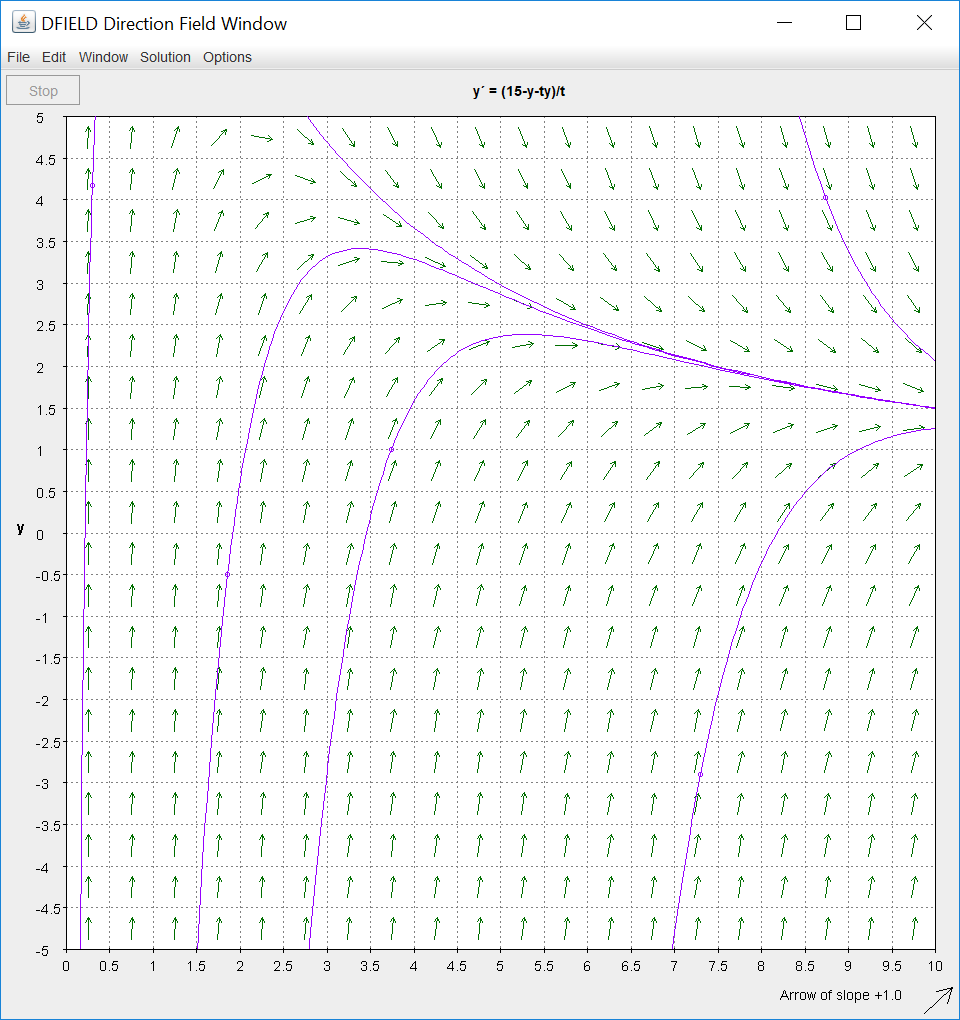
\includegraphics[scale=0.5]{lab1p3p7.PNG}\end{center}
                \item[b)] My conjecture for the limiting behavior as $t \rightarrow \infty$ is that $y$ will approach 1 along the path of the curve.
            \end{enumerate}
        {\bf Problem 8} $(1+t)y'=y(4-y^2)$
            \begin{enumerate}
                \item[a)] $y'=\frac{y(4-y^2)}{1+t}$ \begin{center}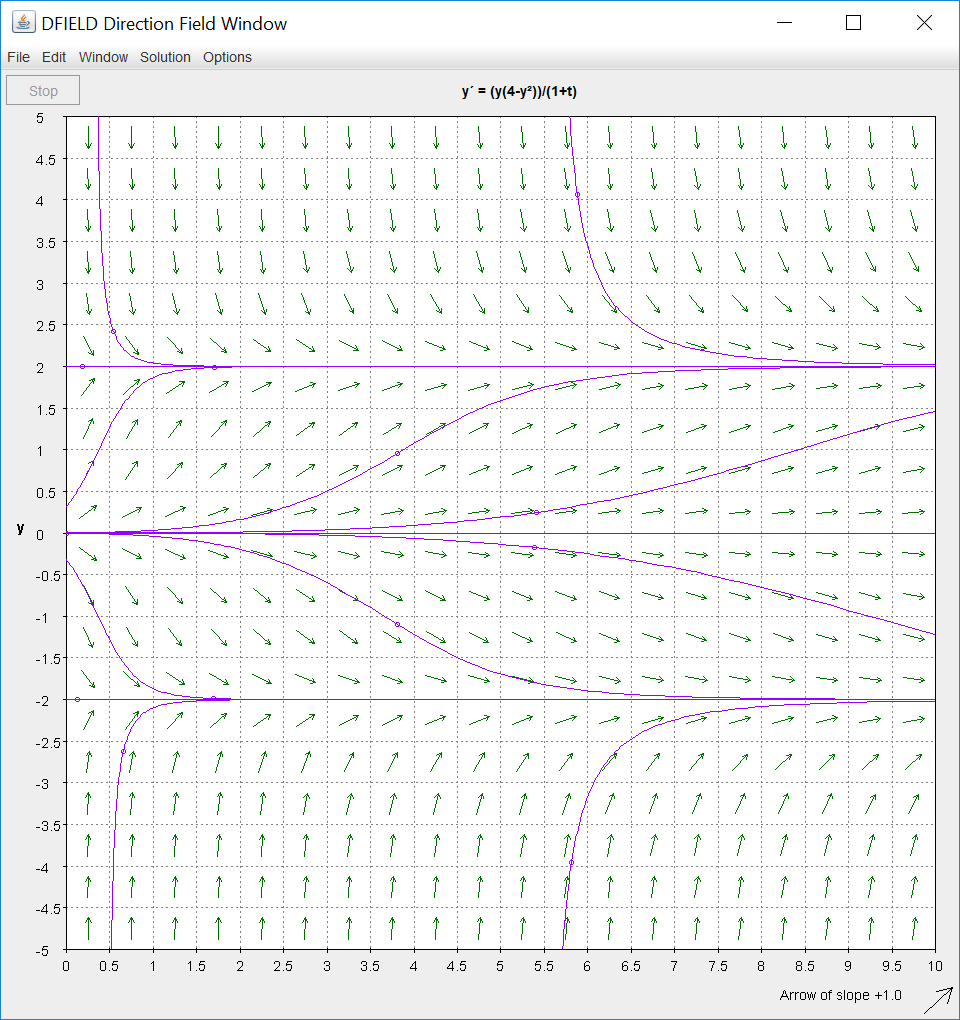
\includegraphics[scale=0.5]{lab1p3p8.PNG}\end{center}
                \item[b)] My conjecture for the limiting behavior as $t \rightarrow \infty$ is that unless $y$ initially starts as 0, in which case it will remain 0, then for $y<0$, then $y=-2$. For $y>0$ then $y=2$.
            \end{enumerate}
        {\bf Problem 9}
            \begin{enumerate}
                \item[1.]    \\ \begin{center}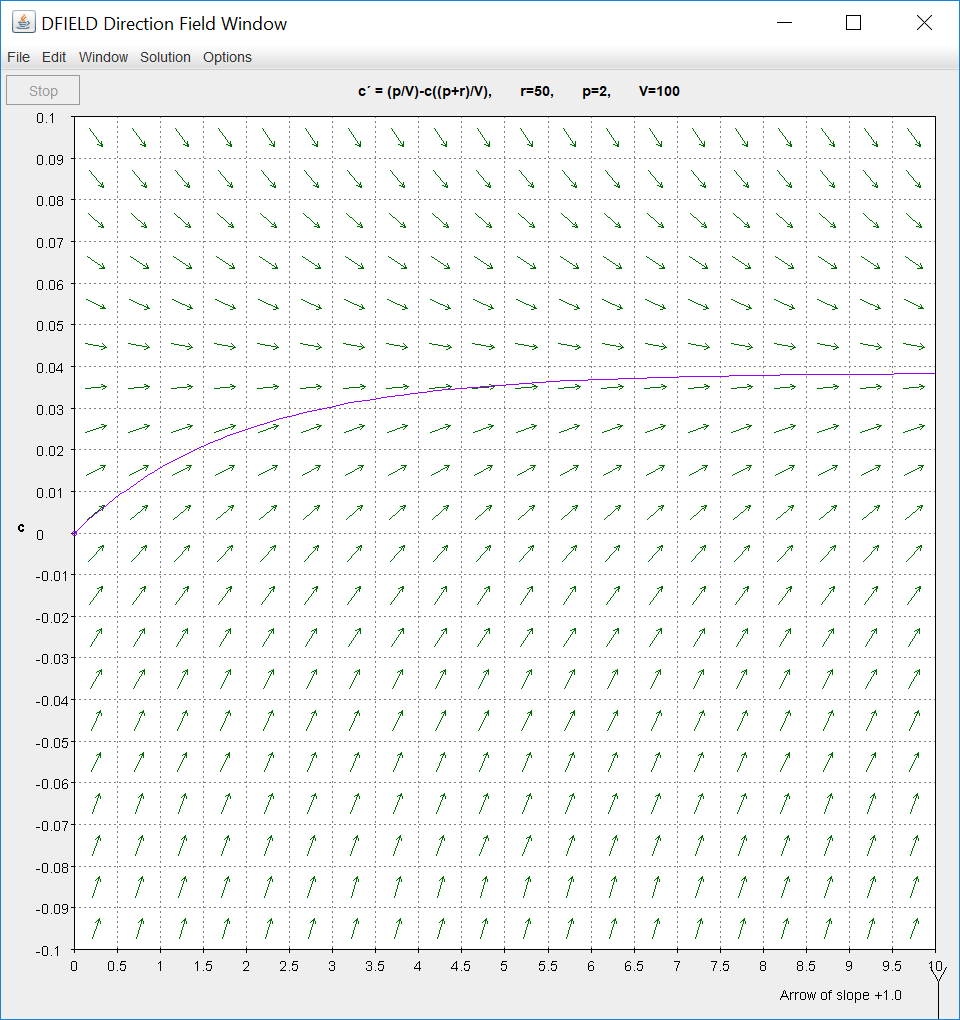
\includegraphics[scale=0.5]{lab1p3p9.PNG}\end{center}
                \item[2.] According to the direction field, it will take approximately 2 years for the concentration to reach 0.025 or $2.5\%$.
                \item[3.] The limiting concentration seems to be 0.04. It appears to take 6 years for the concentration to reach $0.036$ or $3.6\%$. 
            \end{enumerate}
        {\bf Problem 10} When adjusting the numbers to replicate the factory no longer operating while having a concentration of $3.6\%$, it will take less than a year for the concentration to fall below $2.5\%$. Approximately $0.75$ or 9 months out of a year.
            \begin{center}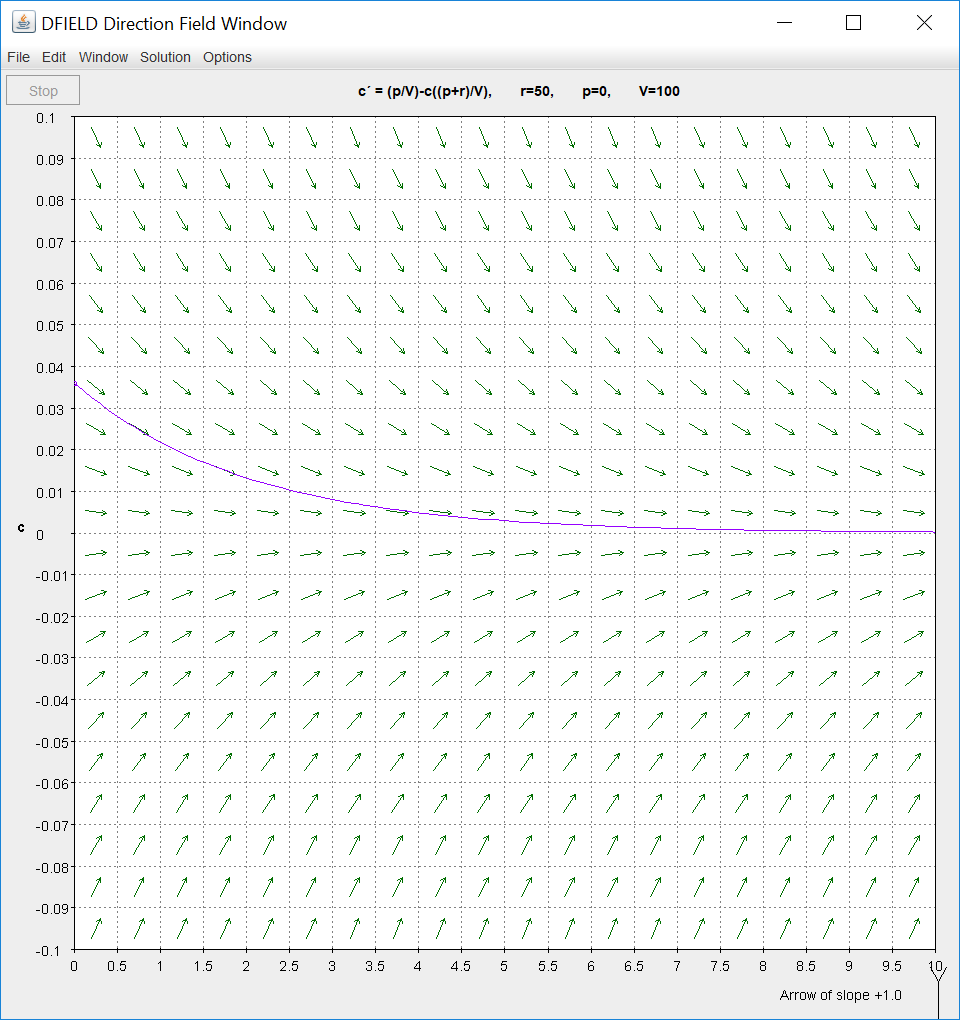
\includegraphics[scale=0.5]{lab1p3p10.PNG}\end{center}
    
    
    \newpage

    \subsection{Linear nth Order Differential Equations}
%provide some kind of introduction to the material here.
    
        \begin{eqnarray*}
            a_n(t)y^{(n)}(t)+a_{n-1}y^{(n-1)}(t)+ ... + a_2(t)y''(t)+a_1(t)y'(t)+a_0y(t)&=&{\^f}(t)\\
            \text{1st order:}\\
            a_1(t)y'(t)+a_0(t)y(t)&=&\^f(t)\\
            y'(t)+\frac{a_0(t)}{a_1(t)}y(t)&=&\frac{\^f(t)}{a_1(t)}\\
            y'(t)+p(t)y&=&f(t).
        \end{eqnarray*}
        Where $f(t)=0$, the solution is {\it homogeneous}. And where $f(t)\neq 0$, the solution is called {\it in-homogeneous}.
        
    \subsection{Variation of Parameters}
%use textbook to provide an introduction as to why this approach is different from separation of variables and why we would use it.
        We'll find both a homogeneous and particular solution when approaching linear nth order differential equations with the variation of parameters approach: $$y_H, y_P.$$
        \begin{eqnarray*}
            y'+p(t)y&=&f(t)=0\\
            y_H'+p(t)y_H&=&0\\
            \frac{dy_H}{dt}&=&-p(t)y_H\\
            \int{\frac{1}{y_H}dy_H}&=&-\int{p(t)dt}\\
            \ln\abs{y_H}&=&-\int{p(t)dt}+c_1\\
            \text{Thus the homogeneous solution looks like:}\\
            y_H&=&ce^{-\int{p(t)dt}}\\
            \text{Now we assume the particular solution takes on a similar form:}\\
            y_P&=&c(t)e^{-\int{p(t)dt}}\\
            \text{We must solve:} && y_P'+p(t)y_P=f(t)\\
            y_P'(t)&=&c(t)e^{-\int{p(t)dt}}[-p(t)]+c'(t)e^{-\int{p(t)dt}}\\
            -c(t)p(t)e^{-\int{p(t)dt}}+c'(t)e^{-\int{p(t)dt}}+c(t)p(t)e^{-\int{p(t)dt}}&=&f(t)\\
            c'(t)e^{-\int{p(t)dt}}&=&f(t)\\
            c'(t)&=&f(t)e^{\int{p(t)dt}}\\
            c(t)&=&\int{f(t)e^{\int{p(t)dt}}dt}\\
            \text{So,}\\
            y_P(t)&=&e^{-\int{p(t)dt}}\int{f(t)e^{\int{p(t)dt}}dt}\\
        \end{eqnarray*}
        
        Now we combine both the particular solution and the homogeneous solution using: 
        $$y(t)=y_H(t)+y_P(t).$$
        And applying: $$y_H'+p(t)y_H=0 \text{ and } y_P'+p(t)y_P=f(t).$$
        Therefore, we get:
        \begin{eqnarray*}
            y'(t)+p(t)y(t)&=&f(t)\\
            (y_H'+y_P')+p(t)(y_H+y_P)&=&f(t)\\
            y_H'+p(t)y_H+y_P'+p(t)y_P&=&f(t)
        \end{eqnarray*}
        
        Finally, the general solution for an nth order differential equation when implementing the Variation of Parameters strategy resembles:         $$y(t)&=&ce^{-\int{p(t)dt}}+e^{-\int{p(t)dt}}\int{f(t)e^{\int{p(t)dt}}dt}$$ 
        
        Practice:
        \begin{enumerate}
            \item[1.] Given that $t\in(0,\pi)$, Solve $y'+(\cot(t))y=t\csc(t)$.\\
            Begin by setting up the homogeneous equation, $y_H'+(\cot(t))y_H=0$, then isolate $y_H'$.
            \begin{eqnarray*}
                \frac{dy_H}{dx}&=&-(\cot(x))y_H\\
                \frac{dy_H}{dt}\cdot\frac{1}{y_H} &=& -\cot(t)\\
                \int{\frac{1}{y_H}dy_H} &=& \int-\cot(t)dt\\
                \ln(y_H) &=& \ln(\sin(t))^{-1})+c &\text{via Substitution.}\\
                e^{\ln(y_H)} &=& e^{\ln(\sin(t))^{-1})+c}\\
                y_H &=& \frac{c}{\sin(t)}
            \end{eqnarray*}
            Then to also introduce the particular solution, guessing that it takes on the same form as the homogeneous solution but with $c$ being a function of $t$.
            \begin{eqnarray*}
                y_P &=& \frac{c(t)}{\sin(t)}\\
                \frac{c'(t)}{\sin(t)} &=& t(\csc(t))\\
                c'(t) &=& t\csc(t)\cdot\sin(t)\\
                c(t) &=&\int t\csc(t)\cdot\sin(t)dt\\
                c(t) &=& \int t dt\\
                c(t) &=& \frac{t^2}{2}\\
                y_{P}&=& \frac{t^2}{2\sin(t)}\\
            \end{eqnarray*}
             Thus, the solution: $y(t)=\frac{c}{\sin(t)}+\frac{t^2}{2\sin(t)}$.
        
            \item[2.] Solve $ty'+5y=7t^2$, given $t>0$.\\
            Begin by dividing through by $t$ in order to simplify the problem, then moving on to the homogeneous equation first.
            \begin{eqnarray*}
                y'+\frac{5}{t}y&=&7t\\
                y_H'+\frac{5}{t}y_H&=&0\\
                y_H'&=&-\frac{5}{t}y_H\\
                \frac{y_H'}{y_H}&=&-\frac{5}{t}\\
                \frac{dy_H'}{dt}\cdot\frac{1}{y_H}&=&-\frac{5}{t}\\
                \int{\frac{1}{y_H}dy_H}&=&\int{-\frac{5}{t}dt}\\
                \ln(y_H)&=&-5\ln(t)+c_1\\
                y_H&=&e^{\ln(t^{-5})+c_1}\\
                y_H&=&c t^{-5}\\
                y_H&=&\frac{c}{t^5}\\
            \end{eqnarray*}
            Making our guess yet again,
            \begin{eqnarray*}
                y_P&=&\frac{c(t)}{t^5}\\
                y_P&=&t^{-5}c(t)\\
                y_P'&=&-5t^{-6}c(t)+t^{-5}c'(t)
            \end{eqnarray*}
            Then inserting this equation into $y_P'+\frac{5}{t}y_H=7t$ we get the following,
            \begin{eqnarray*}
                -5t^{-6}c(t)+t^{-5}c'(t)+\frac{5}{t}\cdot\frac{c(t)}{t^5}&=&7t\\
                t^{-5}c'(t)&=&7t\\
                c'(t)&=&\frac{7t}{t^{-5}}\\
                c'(t)&=&7t^6\\
                c(t)&=&t^7\\
                y_P&=&\frac{t^7}{t^5}=t^2.
            \end{eqnarray*}
        Thus, the solution is $y=\frac{c}{t^5}+t^2$.
        
        \item[3.] Solve $y'+\frac{y}{x}=xy^2$ using the substitution $z=\frac{1}{y}$ to create a linear differential equation.\\
        Therefore, $z=z[y(x)]$ and thus $\frac{dz}{dx}=\frac{dz}{dy}\cdot\frac{dy}{dx}$. Using this, we get $z'(x)=\frac{-1}{y^2}y'$. Solving this equation for $y'$ yields $y'=-y^2 z'(t)$. We can now use this in place of $y'$ and $y$ within the equation.
        \begin{eqnarray*}
            \int{y'dy}&=&\int{y^2 z'(t)dy}\\
        \end{eqnarray*}
%need to locate this problem and its solution.
        \end{enumerate}
        
    \subsection{Integrating Factor}
!!!!!!!! %use textbook to introduce why this approach is different from the others. what benefit does it provide, why should we use it, and when?
    Another approach to solving nth Order Differential Equations is through the method of Integrating Factors. By using the integrating factor approach, we use the same equation: $y'(t)+p(t)y(t)=f(t)$ but this time we designate a specific factor to multiply through the equation with. We will declare this factor as follows, $$\mu=e^{\int{p(t)dt}}.$$
%add a reason why we selected mu to be this.
    Therefore, $$e^{\int{p(t)dt}}y'(t)+e^{\int{p(t)dt}}p(t)y(t)=e^{\int{p(t)dt}}f(t).$$
%I'm not exactly sure why we do the following thing. so add an explanation later.
    See that, $$\int{e^{\int{p(t)dt}}y(t)dt}&=&e^{\int{p(t)dt}}y'(t)+e^{\int{p(t)dt}}p(t)y(t).$$ Then also, $$\frac{d}{dt}[e^{\int{p(t)dt}}y(t)]=e^{\int{p(t)dt}}f(t).$$
    In this case we have declared the derivative of the function $y(t)$, to be $f(t)$. Now we solve for $y(t)$,
    \begin{eqnarray*}
        e^{\int{p(t)dt}}y(t)&=&\int{e^{\int{p(t)dt}}f(t)dt}\\
        y(t)&=&\frac{\int{e^{\int{p(t)dt}}f(t)dt}+c}{e^{\int{p(t)dt}}}\\
        y(t)&=&\int{e^{\int{p(t)dt}}f(t)dt}\cdot e^{-\int{p(t)dt}}+ce^{-\int{p(t)dt}}
    \end{eqnarray*}
    
    \subsection{Mixing Problems}
%probably just input the actual paper for this.
%could include the example problem. The solution and work to the example problem is in the notebook.

        \begin{enumerate}
            \item {\it A 500 liter tank initially contains 10g of salt dissolved in 200 liters of water. Starting at t=0, water that contains 1/4g of salt per liter is poured into the tank at a rate of 4 liters/min and the mixture is drained from the tank at the rate of 2 liters/min. Find a differential equation for the quantity $Q(t)$ or salt in the tank at time t prior to the time when the tank overflows and find the concentration $K(t)$ (g/liter) of salt in the tank at any such time.}\\ \\
            First note the following numbers:\\
            $v=500 L,\hspace{.25cm} c_0=10 g/L, \hspace{.25cm}f_0=2 L/min, \hspace{.25cm}c_i=\frac{1}{4} g/L, \hspace{.25cm}f_i=4 L/min$\\
            Set up the equation as follows, $f_i c_i = \frac{4 L}{1 min}\cdot\frac{1 g}{4 L} = 1 L/min$. Then also by applying the initial amount of water and the difference of $f_i-f_0$, we get $v(t)=200+2t$. By this, the weight equation becomes $w'(t)+\frac{1}{100+t}w(t)=1$. In this case, $p(t)=\frac{1}{100t}$. Therefore, $\mu=e^{\int{p(t)dt}}=e^{\ln{(100+t)}}=100+t$.\\
            \begin{eqnarray*}
                (100+t)w'(t)+(100+t)\frac{1}{100+t}w(t)&=&(100+t)\\
                \frac{d}{dt}[(100+t)w(t)]&=&(100+t)\\
                (100+t)w(t)&=&\int{(100+t)dt}\\
                (100+t)w(t)&=&100t+\frac{t^2}{2}+c\\
                w(t)&=&\frac{100t+\frac{t^2}{2}+c}{(100+t)} = Q(t)
            \end{eqnarray*}
            Notice then, $$K(t)=\frac{Q(t)}{\text{volume}}=\frac{100t+\frac{t^2}{2}+c}{(100+t)\cdot 500}.$$
%add the solution to c found on mathematica file. also help to double check solution from mathematica in order to confirm that this will work.
            
            \item {\it Tank 1 initially contains 100 gal of pure ethanol. Pure water flows into this tank at a rate of 10 gal/min. The perfectly mixed solution flows out of the tank at the same rater, and into Tank 2. Tank 2 initially contains 200 gal of pure water. The perfectly mixed solution leaves Tank 2 at 10 gal/min. Find the quantity or ethanol in each tank, $Q_1(t)$ and $Q_2(t)$. When does Tank 2 reach its maximum level of ethanol?}\\ \\
            $v_1=100 L\text{  pure ethanol},\hspace{.25cm} f_{i1}=10 gal/min,\hspace{.25cm} c_{i1}=0\text{  pure water},\hspace{.25cm} f_{01}=10 gal/min$\\
            $v_2=200 L\text{  pure water},\hspace{.25cm} f_{i2}=10 gal/min,\hspace{.25cm} c_{i2}=100\text{  pure ethanol},\hspace{.25cm} f_{02}=10 gal/min$\\
            Beginning with Tank 1: $$f_{i1}c_{i1}=10\cdot0 = 0.$$
            Thus,
            \begin{eqnarray*}
                w_1'(t)+\frac{10}{100}w_1(t)&=&0\\
                w_1'(t)+\frac{1}{10}w_1(t)&=&0
            \end{eqnarray*}
            Use integrating factor to solve this equation.\\
            $p(t)=\frac{1}{10}$, therefore $\mu=e^{\int p(t)dt}=e^{\frac{t}{10}}$.
            \begin{eqnarray*}
            e^{\frac{t}{10}}w_1'(t)+e^{\frac{t}{10}}(\frac{1}{10})w_1(t)&=&0\\
            \frac{d}{dt}[e^{\frac{t}{10}}w_1(t)]&=&0\\
            e^{\frac{t}{10}}w_1(t)&=&\int{0dt}\\
            e^{\frac{t}{10}}w_1(t)&=&0+c\\
            w_1(t)&=&\frac{c}{e^{\frac{t}{10}}} =ce^{-\frac{t}{10}}\\
            w_1(t)&=&100e^{-\frac{t}{10}}
            \end{eqnarray*}
            
            Now onto Tank 2: $$f_{i2}c_{i2}=100\cdot10 = 1000.$$
            Thus,
            \begin{eqnarray*}
                w_2'(t)+\frac{10}{200}w_2(t)&=&10e^{-\frac{t}{10}}
            \end{eqnarray*}
            Using integrating factor with $p(t)=\frac{10}{200}$, we get $\mu=e^{\int p(t)dt}=e^{\frac{t}{20}}$.
            \begin{eqnarray*}
            e^{\frac{t}{20}}w_2'(t)+e^{\frac{t}{20}}(\frac{1}{20})w_2(t)&=&e^{\frac{t}{20}}(10e^{-\frac{t}{10}})\\
            \frac{d}{dt}[e^{\frac{t}{20}}w_2(t)]&=&e^{\frac{t}{20}}10e^{-\frac{t}{10}}\\
            e^{\frac{t}{20}}w_2(t)&=&\int{e^{-\frac{t}{20}}dt}\\
            e^{\frac{t}{20}}w_2(t)&=&-20e^{-\frac{t}{20}}+c\\
            w_2(t)&=&\frac{-20e^{-\frac{t}{20}}+c}{e^{\frac{t}{20}}}\\
            w_2(t)&=&e^{-\frac{t}{20}}(-20e^{-\frac{t}{20}}+c)
            \end{eqnarray*}
            With c=220. 
%answer the actual question here at some point. the actual question is not answered yet.
        \end{enumerate}
    
    \subsection{Solutions of nth Order, Constant Coefficient, Linear, Homogeneous ODEs/IVPs}
        {\bf Theorem 1} {\it Let $y_1,...,y_n$ be linearly independent solutions of the homogeneous equation} 
            \begin{eqnarray*}
            y^{(n)}+a_{n-1}y^{(n-1)}+&...&a_1y^{(1)}+a_0y=0 &(1)
            \end{eqnarray*}
            {\it If Y is any solution whatsoever of (1) on $\mathbb{R}$, then there exist numbers $c_1,...,c_n$ such that $$Y(t)=c_1y_1(t)+...+c_n y_n (t)$$ for all $t\in\mathbb{R}$.}\\
        {\bf Theorem 2} {\it (1) has a unique solution on $\mathbb{R}$ that satisfies the n conditions $$y(a)=b_0,\hspace{.5cm}y'(a)=b_1,\hspace{.5cm}...\hspace{.5cm},\hspace{.5cm} y^{(n-1)}(a)=b_{(n-1)}.$$}

    \subsection{Achieving Linearly Independent Solutions For nth Order Equations}
    Here we consider constant coefficient homogeneous differential equations of the form 
    $$y^{(n)}+a_{(n-1)}y^{(n-1)}+..+a_1 y^{(1)}+a_0 y=0.$$
    Assuming the solution $y=e^{rt}$, we compute the auxiliary equation: $$r^n +a_{n-1} r^{n-1} +...+a_1r+a_0 =0.$$
    Now per the Fundamental Theorem of Algebra, we are ensured the existence of $n$ solutions. If these roots are all distinct, i.e. $$(r-r_1)(r-r_2)...(r-r_n)=0,$$
    then it can be shown that the solutions $y_i=e^{r_i t}$ are all linearly independent. So the general solution is $$y(t)=c_1 e^{r_1 t}+...+c_1 e^{r_n t}.$$
    If we have repeated roots, then we must achieve linear independence in some alternate manner. For convenience, we can define the general differential equation using the operators $D^n =\frac{d^n}{dt^n}$, for $n=1,2,...$. Then we rewrite the equation as
    \begin{eqnarray*}
        D^n y+a_{n-1}D^{n-1}y+...+a_1 Dy+a_0 y&=&0, \text{ or}\\
        (D-r_1)(D-r_2)...(D-r_n)y&=&0.
    \end{eqnarray*}
    Now assume there are $k$ repeated roots. Then we can focus on that portion of the differential equation:
    \begin{eqnarray*}
        (D-r_1)^k y &=& 0, \text{ or}\\
        \underbrace{(D-r_1)...(D-r_1)}_k y&=&0.
    \end{eqnarray*}
    At this point, we can identify only one independent solution $y_1=e^{r_1 t}$. We still need to find the remaining $k-1$ solutions. To do so, we try the solution $y=u(t)e^{r_1 t}$ in our differential equation, and attempt to find the coefficient $u(t)$:
    $$\underbrace{(D-r_1)...(D-r_1)}_k u(t)e^{r_1 t} =0.$$
    Note that
    \begin{eqnarray*}
        (D-r_1)u(t)e^{r_i t} &=& Du(t)e^{r_1 t}-r_1 u(t)e^{r_1 t}\\
        &=& u'(t)e^{r_1 t}+u(t)r_1e^{r_1 t}-r_1 u(t)e^{r_1 t}\\
        &=&u'(t)e^{r_1 t}.
    \end{eqnarray*}
    We then apply the next operator to this function, and note that:
    $$(D-r_1)^2 = (D-r_1)(u'(t)e^{r_1 t}=...=u''(t)e^{r_1 t}.$$
    Proceeding inductively, we find that
    $$(D-r_1)^k = u^{(k)}(t)e^{r_1 t}.$$
    We set this equal to zero, as required by the differential equation:
    \begin{eqnarray*}
        u^{(k)}(t)e^{r_1 t} &=& 0 \Rightarrow\\
        u^{(k)}(t)&=&0.
    \end{eqnarray*}
    At this point we can integrate $k$ times to solve for $u(t)$:
    $$u(t)=c_0+c_1 t+c_2 t^2 +...+c_{k-2}t^{k-2}+c_{k-1}t^{k-1}.$$
    As such, we see the repeated portion(s) of the general solution to the differential equation is comprised of $k$ linearly independent solutions:
    \begin{eqnarray*}
        y(t)&=&u(t)e^{r_1 t}\\
        &=&(c_0+c_1 t+c_2 t^2 +...+c_{k-2} t^{k-2} +c_{k-1} t^{k-1})e^{r_1 t}\\
        &=&\underbrace{c_0 e^{r_1 t}+c_1 t e^{r_1 t}+c_2 t^2 e^{r_1 t}+...+c_{k-2} t^{k-2} e^{r_1 t}+c_{k-1} t^{k-1}e^{r_1 t}}_k .
    \end{eqnarray*}
    This portion is then combined with the other $n-k$ linearly independent solutions, for the full general solution.\\
    (Via Trent Kull).
    
    \subsection{2nd Order, Linear, Constant Coefficient, Homogeneous Equations}
    When solving differential equations of the form:
    $$y''(t)+a_1 (t) y'(t)+a_0(t)y(t)=f(t)=0,$$
    such that $a_1(t), a_0(t)\in\mathbb{R}$, the equation simplifies to
    $$y''(t)+by'(t)+cy(t)=0,$$
    and there are three resulting cases. To find these, we begin by making a guess that the general solution will take on a form that follows:
    \begin{eqnarray*}
        y(t)&=&e^{rt}\\
        y'(t)&=&re^{rt}\\
        y''(t)&=&r^2 e^{rt}.
    \end{eqnarray*}
    By this, we adjust the equation to,
    \begin{eqnarray*}
        r^2 e^{rt}+b re^{rt}+ce^{rt}&=&0 \Rightarrow\\
        r^2+br+c&=&0\\
        r&=&\frac{-b\pm \sqrt{b^2-4(1)(c)}}{2(1)}.
    \end{eqnarray*}
    We therefore find the division into three different cases of solution sets.\\
    
    \underline{Case 1:} Solutions are Real and Distinct. Thus, $r_1\neq r_2$.\\
    In this case, the resulting solutions maintain their original form:
    \begin{eqnarray*}
        \begin{rcases}
        y_1(t)&=&e^{r_1 t}\\
        y_2(t)&=&e^{r_2 t}
        \end{rcases}
        y(t)=c_1 y_1(t)+c_2 y_2(t)
    \end{eqnarray*}
    Thus,
    \begin{eqnarray*}
        y_1''(t)+by_1'+cy_1&=&0\\
        y_2''(t)+by_2'+cy_2&=&0
    \end{eqnarray*}
    And because $y=y_1+y_2$, we get
    $$(y_1''+y_2'')+b(y_1'+y_2')+c(y_1+y_2)=0.$$
    
    \underline{Case 2:} Solutions are Real but Repeated. Thus, $r_1=r_2$.\\
    In this case, the solutions are ``not different enough". So we must find another solution and because of this, there is more work required with this case.\\
%add this later

    \underline{Case 3:} Solutions are Complex and Distinct. Thus, $r_{1,2}=\alpha\pm i\beta,$ where $\beta\neq 0$.\\
    
\end{document}